\section{Introduction}

With the flourishing development of e-commerce platforms, online shopping has become part of people's lives. In order to further stimulate online consumption, e-commerce platforms arrange various promotion campaigns on special days, such as Black Friday~\cite{2013Black} in Western countries and Double Eleven in China~\cite{huang2019x}. Due to the fact that online promotions are too numerous, people can not get promotion information for the first time, some intermediate platforms have emerged in the market, such as Groupon~\cite{groupon} and Dealmoon~\cite{dealmoon}. These platforms help users sort out the hot deals of various e-commerce platforms, saving the user's shopping time.

However, sometimes even users know those promotion, they found that their purchase fails to meet the spending threshold to use a coupon or to enjoy the delivery service. In this situation, users will intentionally ask their friends or look for other person on the social networks to place one order together in order to meet the threshold. Because all the e-commerce platforms support only one shipping address for one order, when multiple users place an order together, one of the users will inevitably receive all the products first and then distribute them to others respectively. These complex processes are unreliable and time-consuming for consumers.

What is even more damaging to consumers' motivation to shopping is that e-commerce promotion activities have become increasingly complicated in recent years. For example, during the 2020 Taobao Double eleven, the platform prolonged the promotional period. This change might aim at bringing more benefits and convenience to consumers, but indeed imposes extra workloads to them, since multiple complex coupons rules change on a daily basis. As a matter of fact, consumers complains that it takes much time to decipher the coupon rules in order to enjoy the event's maximum benefit~\cite{2020} ~\cite{double11}.
\begin{figure}[t] 
\centering %图片居中
		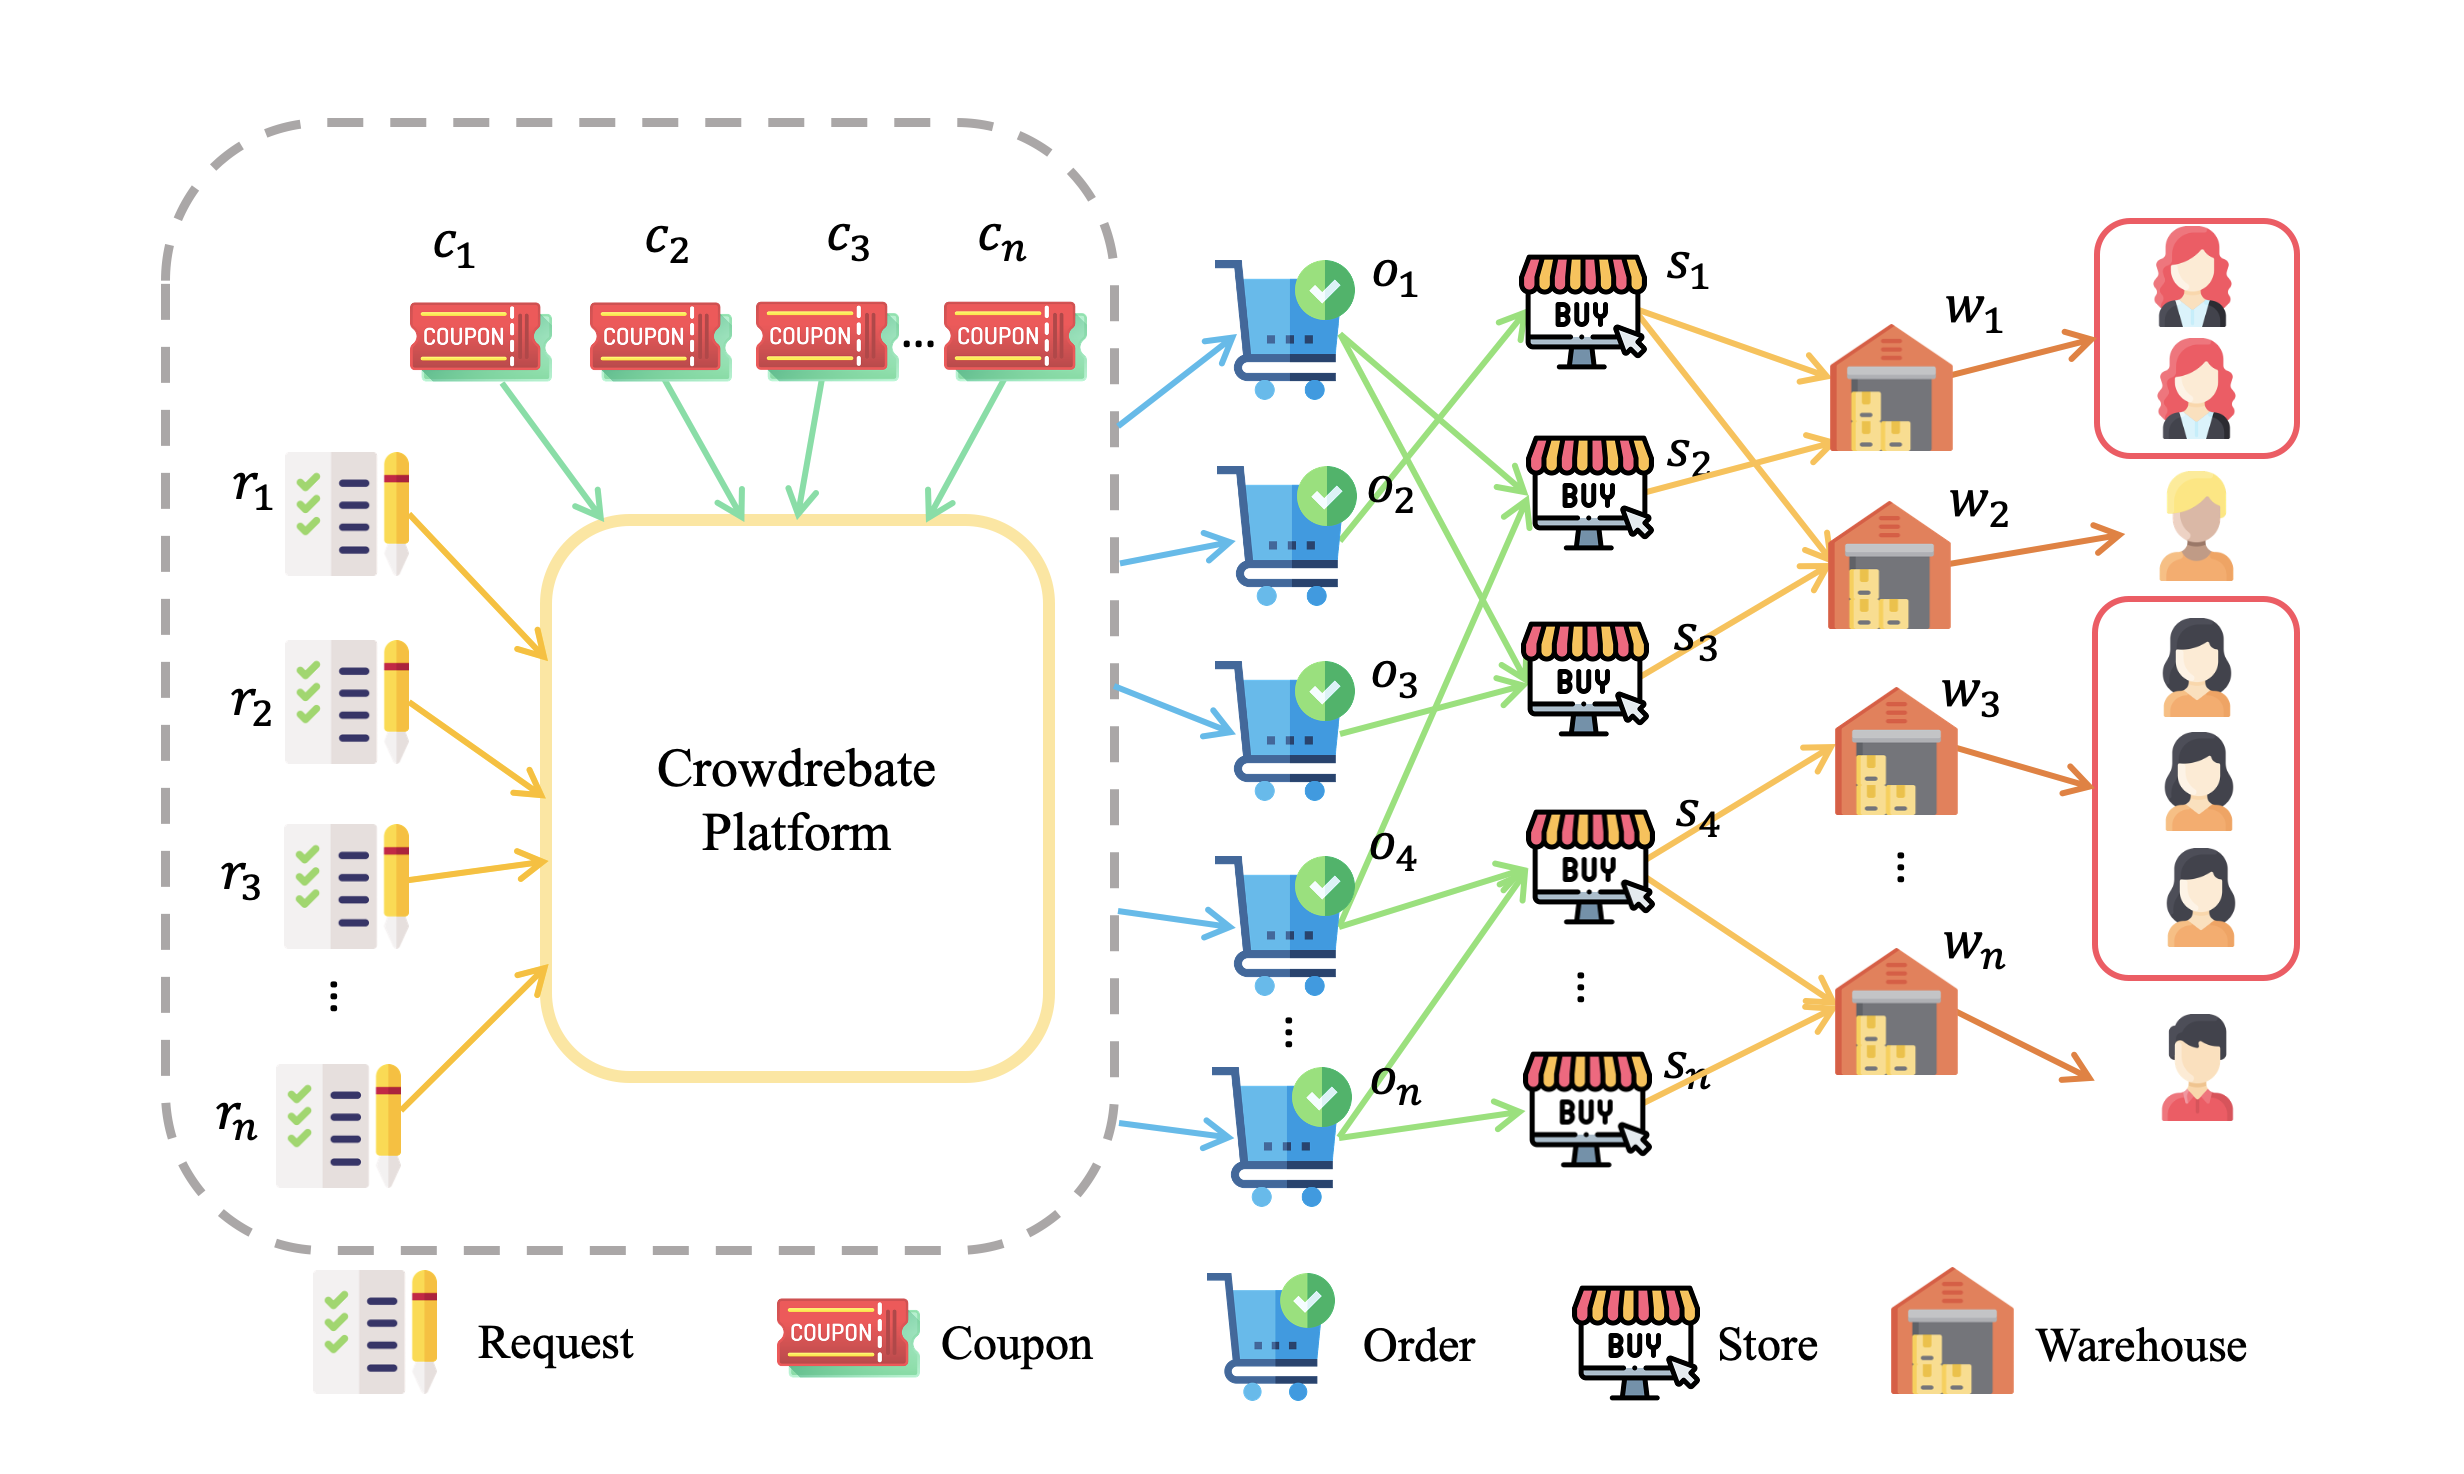
\includegraphics[width=0.4\textwidth]{../figure/crowdrebate process.png} %插入图片,[]中设置图片大小,{}中是图片文件名
	\caption{The operation process of crowdrebate} %最终文档中希望显示的图片标题
	\label{fig:Crowdrebate} %用于文内引用的标签
	\end{figure}

Under these circumstances, our demo-Crowdrebate firmly grasps consumer's pain point. Crowdrebate collects users’
purchasing requests and group their requests into orders to
maximize total benefit. Meanwhile, we give the exposure of online retailers' promotions so that more users would participate in promotions. To summarize, not only do we dedicate ourselves to help users get more benefits, we also devote ourselves to help e-commerce platforms fill more orders, increase platforms’ revenue, and ultimately achieve a bilateral win-win situation.

Our platform operates as follows~\ref{fig:Crowdrebate}. Users can post their requirements on our platform. Each requirement corresponds to the e-commerce platform they would like to order from, such as the specific stores, specific products, and prices, as well as the expected period of placing order. Based on the received requests, we will make an order association and match the coupons we crawled from the e-commerce platform to maximize each order's rebate. Owing to the fact that we place the orders for consumers, the products will first be sent to our warehouses from the online stores, and then we will distribute the products to the according users.

Thus, our demo has three core components: 
\begin{itemize}
	\item Users can publish their needs, our platform collects the demands and crawls online coupons to make patchwork combinations;
	\item Users can view the latest coupons of e-commerce platforms and the popular products that users would like to buy on the platforms;
	\item Users can view their historical data analysis, such as our service charges and the amount of money we help users to save. Furthermore, we can also provide an API to our partner platforms so that they can see the coupon data (such as the regional distribution of users, favorite stores and products, etc.) of the coupons used on our platform.
\end{itemize}
\begin{figure}[t] 
	\centering %图片居中
	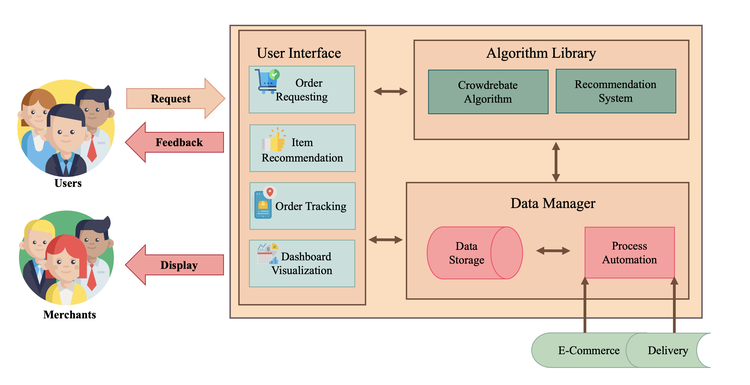
\includegraphics[width=0.4\textwidth]{../figure/ar.png} %插入图片,[]中设置图片大小,{}中是图片文件名
	\caption{The architecture of crowdrebate} %最终文档中希望显示的图片标题
	\label{fig:ar} %用于文内引用的标签
\end{figure}

